\section{Backend}
\label{Backend}
V rámci projektu Tempora jsem zvolil Supabase jako backendové řešení pro správu databáze a autentizaci uživatelů. Supabase nabízí funkcionalitu podobnou Firebase s plnou podporou PostgreSQL, což mi umožňuje efektivně pracovat se strukturovanými daty. Supabase jsem si vybral převážně kvůli jednoduché implementaci do Nuxt frameworku a automatické údržbě databázového backendu, která eliminuje nutnost správy vlastních serverů, čímž výrazně urychlila vývoj projektu.

\subsection{Logické soubory - JavaScript}
I když JavaScript není úplně backendový jazyk, zmíním ho právě v této kapitole, protože až na výjimky obsluhuje operace, které nejsou uživatelem vidět v grafickém rozhraní. Veškeré JavaScriptové soubory mám ve složce composables. 

\textbf{\textit{UseSupabase.js}} - soubor, ve kterém jsou požadavky na databázi týkající se uživatelských dat, jako je jméno, uložené osy a také časové osy, jako je vytvoření časové osy, její aktualizace nebo smazání.

Druhým souborem pro obsluhu databáze je \textit{\textbf{supabaseItem.js}}. Zde jsou veškeré databázové dotazy týkající se jednotlivých událostí, od jejich načítání až po smazání. Tyto soubory využívají supabaseClient pro komunikaci s databází.

Aby se jednotlivé události správně ukládaly do databáze, je nejprve nutné je upravit do správného tvaru, převést roky na milisekundy atd. \textbf{\textit{ItemManipulation.js}} zařizuje právě tyto úkony a rozhoduje podle parametrů, které dostane, do jakých řádků se musí jaké údaje uložit, aby časová osa vypadala tak, jak uživatel potřebuje.

U mé komponenty časové osy je nedílnou součástí \textbf{\textit{timelineFeatures.js}}. Tento soubor slouží k poskytnutí a aktualizaci správně zobrazených dat na časové ose a funkcionalitě jednotlivých ovládacích prvků, jako je přibližování, posouvání nebo zobrazovaný rok při najetí kurzoru nad časovou osu.

Posledním souborem je \textbf{\textit{state.js}}. Tento soubor byl původně vytvořen pouze k uchování stavu postranního menu, ale později do něj bylo začleněno i přepínání režimů pro nastavení, zobrazení a úpravy časové osy.

\subsection{Ověření uživatele}
Supabase používá k autentikaci základní tabulku auth.users, kterou automaticky spravuje. Do této tabulky se vždy po registraci s e-mailem a heslem přidá nový uživatel a na jeho e-mailovou adresu se odešle automaticky generovaný odkaz pro potvrzení. 

V aplikaci jsem chtěl mít registraci a přihlášení nepovinné. Uživatel tedy nepotřebuje účet, aby procházel veřejné osy, pouze mu chybí možnost tvorby nových os a ukládání svých oblíbených časových os. 
\cite{Nuxt-Auth, Supabase-Middleware-fix, guest-logged-in-access-Chat}  

\subsection{Databázová struktura}
Pro práci se všemi daty využívám čtyři SQL tabulky: timelines, items, user\_profiles, bookmarks a jednu předgenerovanou auth.users. Tyto tabulky jsou vzájemně propojené a interagují s webovou stránkou, viz obrázek \ref{fig:Struktura tabulek}.

\begin{figure}[h]
    \centering
    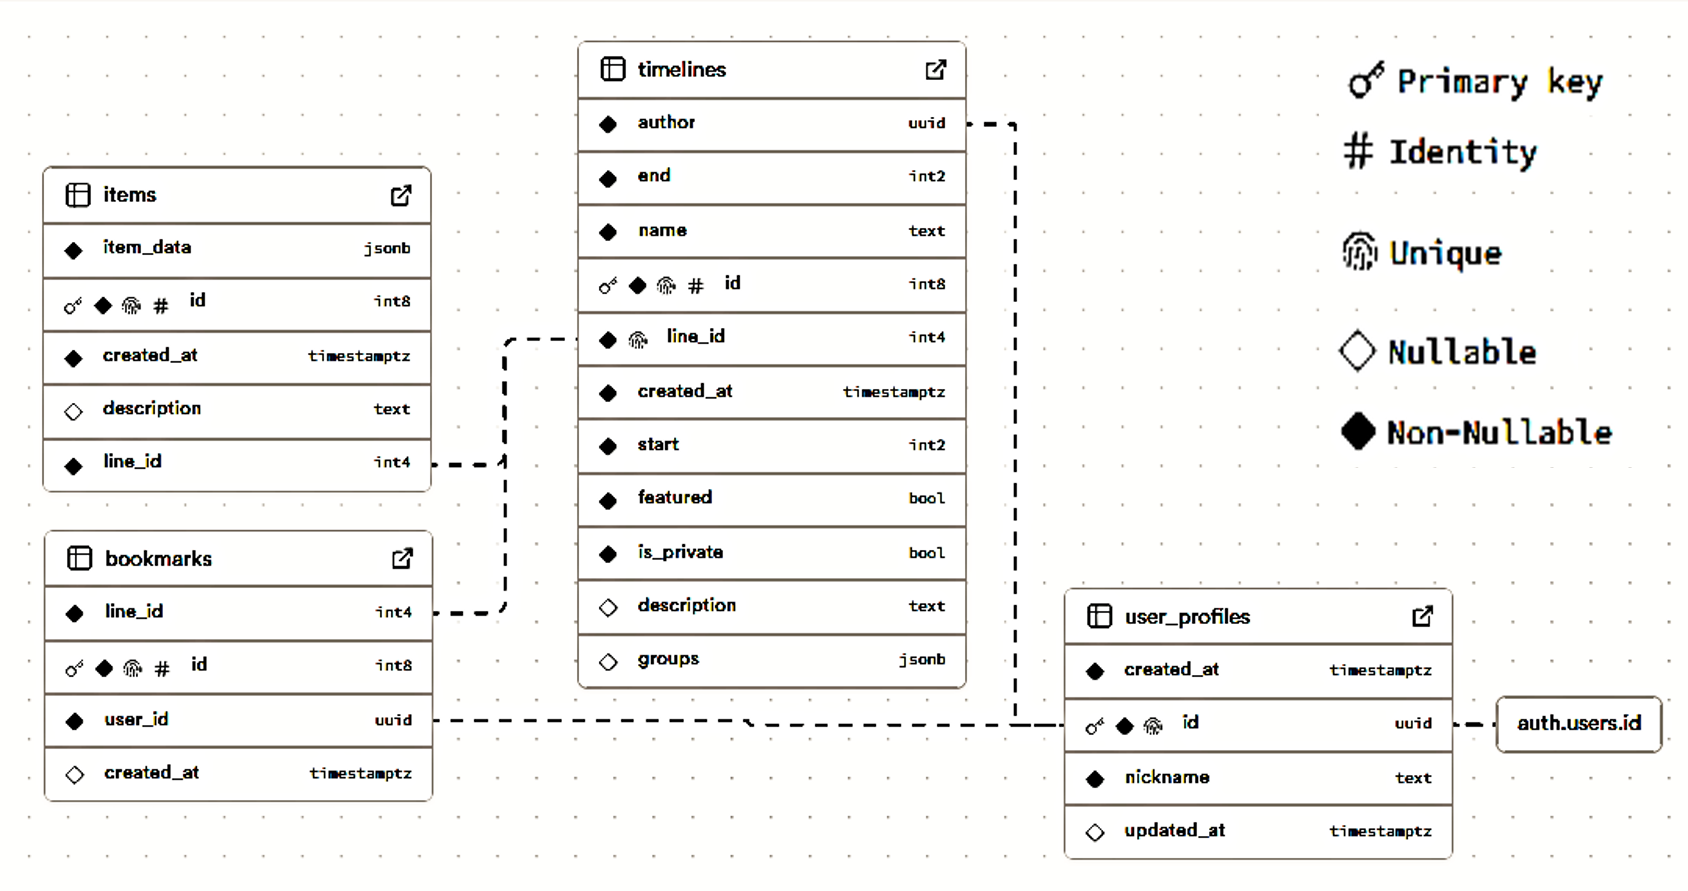
\includegraphics[width=1\linewidth]{Images/SupabaseStructure.png}
    \caption{Struktura tabulek z vizualizace v Supabase, legenda značek}
    \label{fig:Struktura tabulek}
\end{figure}

\subsubsection{Tabulka – timelines}
V centru celého systému stojí tabulka timelines, ve které jsou uložena všechna data, která se samotné časové osy týkají. Hlavními částmi jsou id, name – jméno dané časové osy, start a end, určující počátek a konec zobrazovaného období, line\_id, obsahující šestimístné číslo, které určuje odkaz na danou osu a zároveň slouží k propojení s dalšími tabulkami. \newpage
Featured je booleanová proměnná, která určuje, zda se daná osa zobrazí pro všechny uživatele na stránce v sekci „Vybrané“. Is\_private si nastavuje každý uživatel sám – určuje možnost návštěv autorovi osy jinými uživateli, více v sekci \ref{policies} \textit{Tabulková pravidla (policies)}. Uživatel si v časové ose také může nastavit jména jednotlivých řádků, což se ukládá ve formátu jsonb \cite{jsonb} do groups, a vlastní popis osy, který je uložen v description. 

\subsubsection{Tabulka – items}
Tabulka items zabezpečuje správné uložení jednotlivých událostí. Je propojená s tabulkou timelines pomocí cizího klíče line\_id. Obsahuje údaj o vytvoření a detailnější popis dané události, který má v databázi formát obyčejného textu, i když jsou v něm uloženy prvky v HTML syntaxi (\texttt{\textless h3\textgreater Nadpis \textless /h3\textgreater}).

Nejsložitější strukturou je pak určitě jsonb item\_data, který obsahuje všechny potřebné informace vyžadované knihovnou vue-timeline-chart ke správnému umístění na osu, viz ukázka \ref{item_data}.
Události jsem rozdělil na dva typy – kontextové a normální. Normální událost se skládá ze tří řádků: hlavní části, vedlejší a detailu (korespondující s označením řádků v kapitole \ref{Komponent časové osy}). Bohužel knihovna, kterou jsem využíval, neumožňuje přidat jednu událost na více řádků, proto jsem normální událost musel rozdělit do tří částí. Každý předmět má své unikátní id, začátek a konec, jméno, které se zobrazuje v časové ose, barvu nastavenou jako cssVariable, group označující řádek, kam bude umístěn, a poslední tag, podle kterého se sjednocují zmíněné tři části normální události. Kontextová událost je velice intuitivní, skládá se jen z jedné hlavní části a má všechny zmíněné proměnné stejné, jen tag je u ní vždy roven id.

\begin{lstlisting}[style=JavaScript, firstnumber = 1, caption={item\_data, Supabase items table}, label={item_data}]
{
  "id": 35,
  "end": -473385600000,
  "tag": 35,
  "name": "Osvicenstvi v literature",
  "group": 5,
  "start": -631152000000,
  "cssVariables": {
    "--item-background": "#073E5A"
  }
}
\end{lstlisting}

\subsubsection{Tabulka – user\_profile}
Tato tabulka je propojená se základní tabulkou auth.users.id a stará se o ukládání uživatelského nastavení. Protože jsem nechtěl, aby si jiní uživatelé mohli zobrazit váš e-mail, vytvořil jsem možnost nastavit si vlastní uživatelské jméno (nickname).  

\subsubsection{Tabulka – bookmarks}
Pro zlepšení uživatelského prostředí byla vytvořena tabulka bookmarks, která přidává uživateli funkci uložit si časové osy, které se mu líbily, a umožní mu k nim snadný přístup v sekci „Uložené“. Jsou v ní uložena ID časových os a UUID uživatelů.

\subsection{Tabulková pravidla (policies)}
\label{policies}
U všech svých tabulek mám zapnuté RLS neboli row-level security, které slouží k řízení přístupu k datům na úrovni jednotlivých řádků v tabulkách. Při použití RLS je důležité pečlivě nastavit příslušná pravidla (policies), která definují, kteří uživatelé nebo role mají jaká oprávnění pro čtení, vkládání, aktualizaci a mazání dat. Tato pravidla jsou definována pomocí SQL funkcí, které vracejí logickou hodnotu true nebo false v závislosti na kontextu aktuálního uživatele. V Supabase lze tato pravidla nastavovat přímo v uživatelském rozhraní. 

Například pro tabulku timeline mám nastavená pravidla: přidat novou osu může jen přihlášený uživatel, aktualizovat a mazat data může pouze autor dané časové osy. Pro zobrazení dat mám dvě pravidla – pokud je osa veřejná, nemusím kontrolovat nic. Pokud je ale osa soukromá, je nutné zjistit, zda je daný uživatel autorem, a na základě toho data buď zobrazit, nebo ne.


\begin{figure}[h]
    \centering
    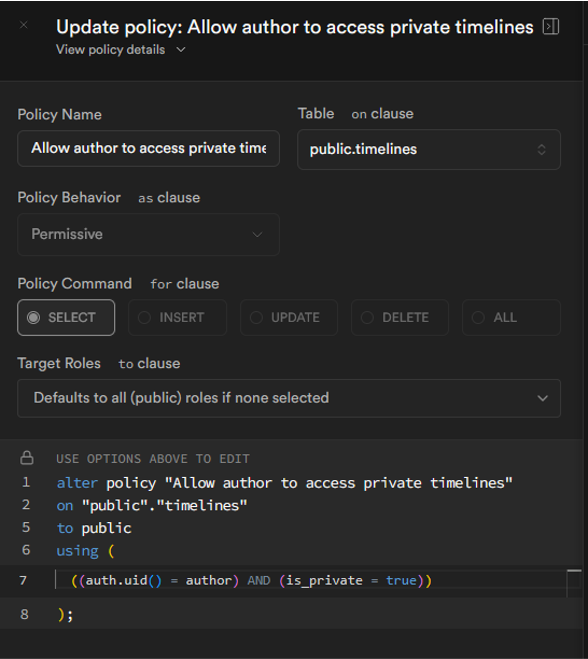
\includegraphics[width=0.45\linewidth]{Images/Policy_example.png}
    \caption{Ukázka nastavení pravidla tabulky v Supabase}
    \label{fig:Policy example}
\end{figure}

Zprvu jsem měl tuto ochranu jen na tabulku timelines, takže pokud by znal nepřihlášený uživatel id nějaké události v soukromé ose, mohl si ji zobrazit, i když k ose jako takové přístup neměl. Tento problém jsem samozřejmě opravil.

\newpage

\subsection{Práce s daty v databázi}
Díky ekosystému Nuxt je práce mezi programem a databází víceméně přímočará. Každá funkce v \textit{useSupabase.js} a \textit{supabaseItem.js} používá pro komunikaci s databází asynchronní funkci useSupabaseClient(), do které se zadají požadované SQL příkazy. Každá funkce má také návratovou hodnotu – ta může obsahovat samotná data při načítací funkci nebo odpověď databáze, buď o provedení, nebo o chybě, která nastala.

\subsection{Ukládání událostí}
Ukládání událostí je asi nejtěžší operace, při které záleží na různých parametrech, aby fungovala správně. Celý tento cyklus začíná v \textit{itemEditComp.vue}, kde se po zmáčknutí tlačítka „Uložit změny“ zavolá funkce saveChanges, která zkontroluje správnost zadaných roků, a pokud je vše správně, zavolá funkci handleItemUpdate z \textit{itemManipulation.js} se všemi parametry. Tato funkce se skládá ze tří částí: ukládání nově vytvořených částí, aktualizace již vytvořených a smazání nepotřebných událostí. Funkce se rozhoduje na základě parametrů od uživatele v porovnání s daty načtenými z databáze. Například pokud normální událost již měla v databázi uloženou hlavní a sekundární část a uživatel sekundární smazal, funkce zavolá \textit{updateItem}, aktualizuje hlavní část a sekundární smaže pomocí \textit{removeItem} z \textit{supabaseItem.js}. 

Při tvorbě nové části události je důležité podívat se na poslední použité ID a vytvořit další tak, aby se žádné neopakovalo. Dalším úskalím při tvorbě nové události je její uložení do správného řádku na základě parametrů contextType a isBottom, což řeší tato část kódu – ukázka \ref{groups}.      

\begin{lstlisting}[style=JavaScript, firstnumber = 154, caption={Handle update, itemManipulation.js}, label={groups}]
const mainGroup = contextType
  ? isBottom
    ? 8 : 1
  : isBottom
    ? 5 : 2;

  const secondaryGroup = isBottom ? 6 : 3;
  const detailGroup = isBottom ? 7 : 4;
\end{lstlisting}

Při tvorbě úplně nové události z postranního menu v \textit{SidebarComb.vue} používám stejnou funkci saveChanges, pouze je nastaven parametr pomocí query z přesměrování: \texttt{const creatingNew = ref(route.query.creatingNew === 'true');}.
